\appendix{Представление графического материала}

Графический материал, выполненный на отдельных листах,
изображен на рисунках А.1--А.\arabic{числоПлакатов}.
\setcounter{числоПлакатов}{0}

\renewcommand{\thefigure}{А.\arabic{figure}} % шаблон номера для плакатов

\begin{landscape}

\begin{плакат}
    \includegraphics[width=0.82\linewidth]{RAMKA_VKR.eps}
    \заголовок{Сведения о ВКРБ}
    \label{RAMKA_VKR.eps:image}      
\end{плакат}

\begin{плакат}
    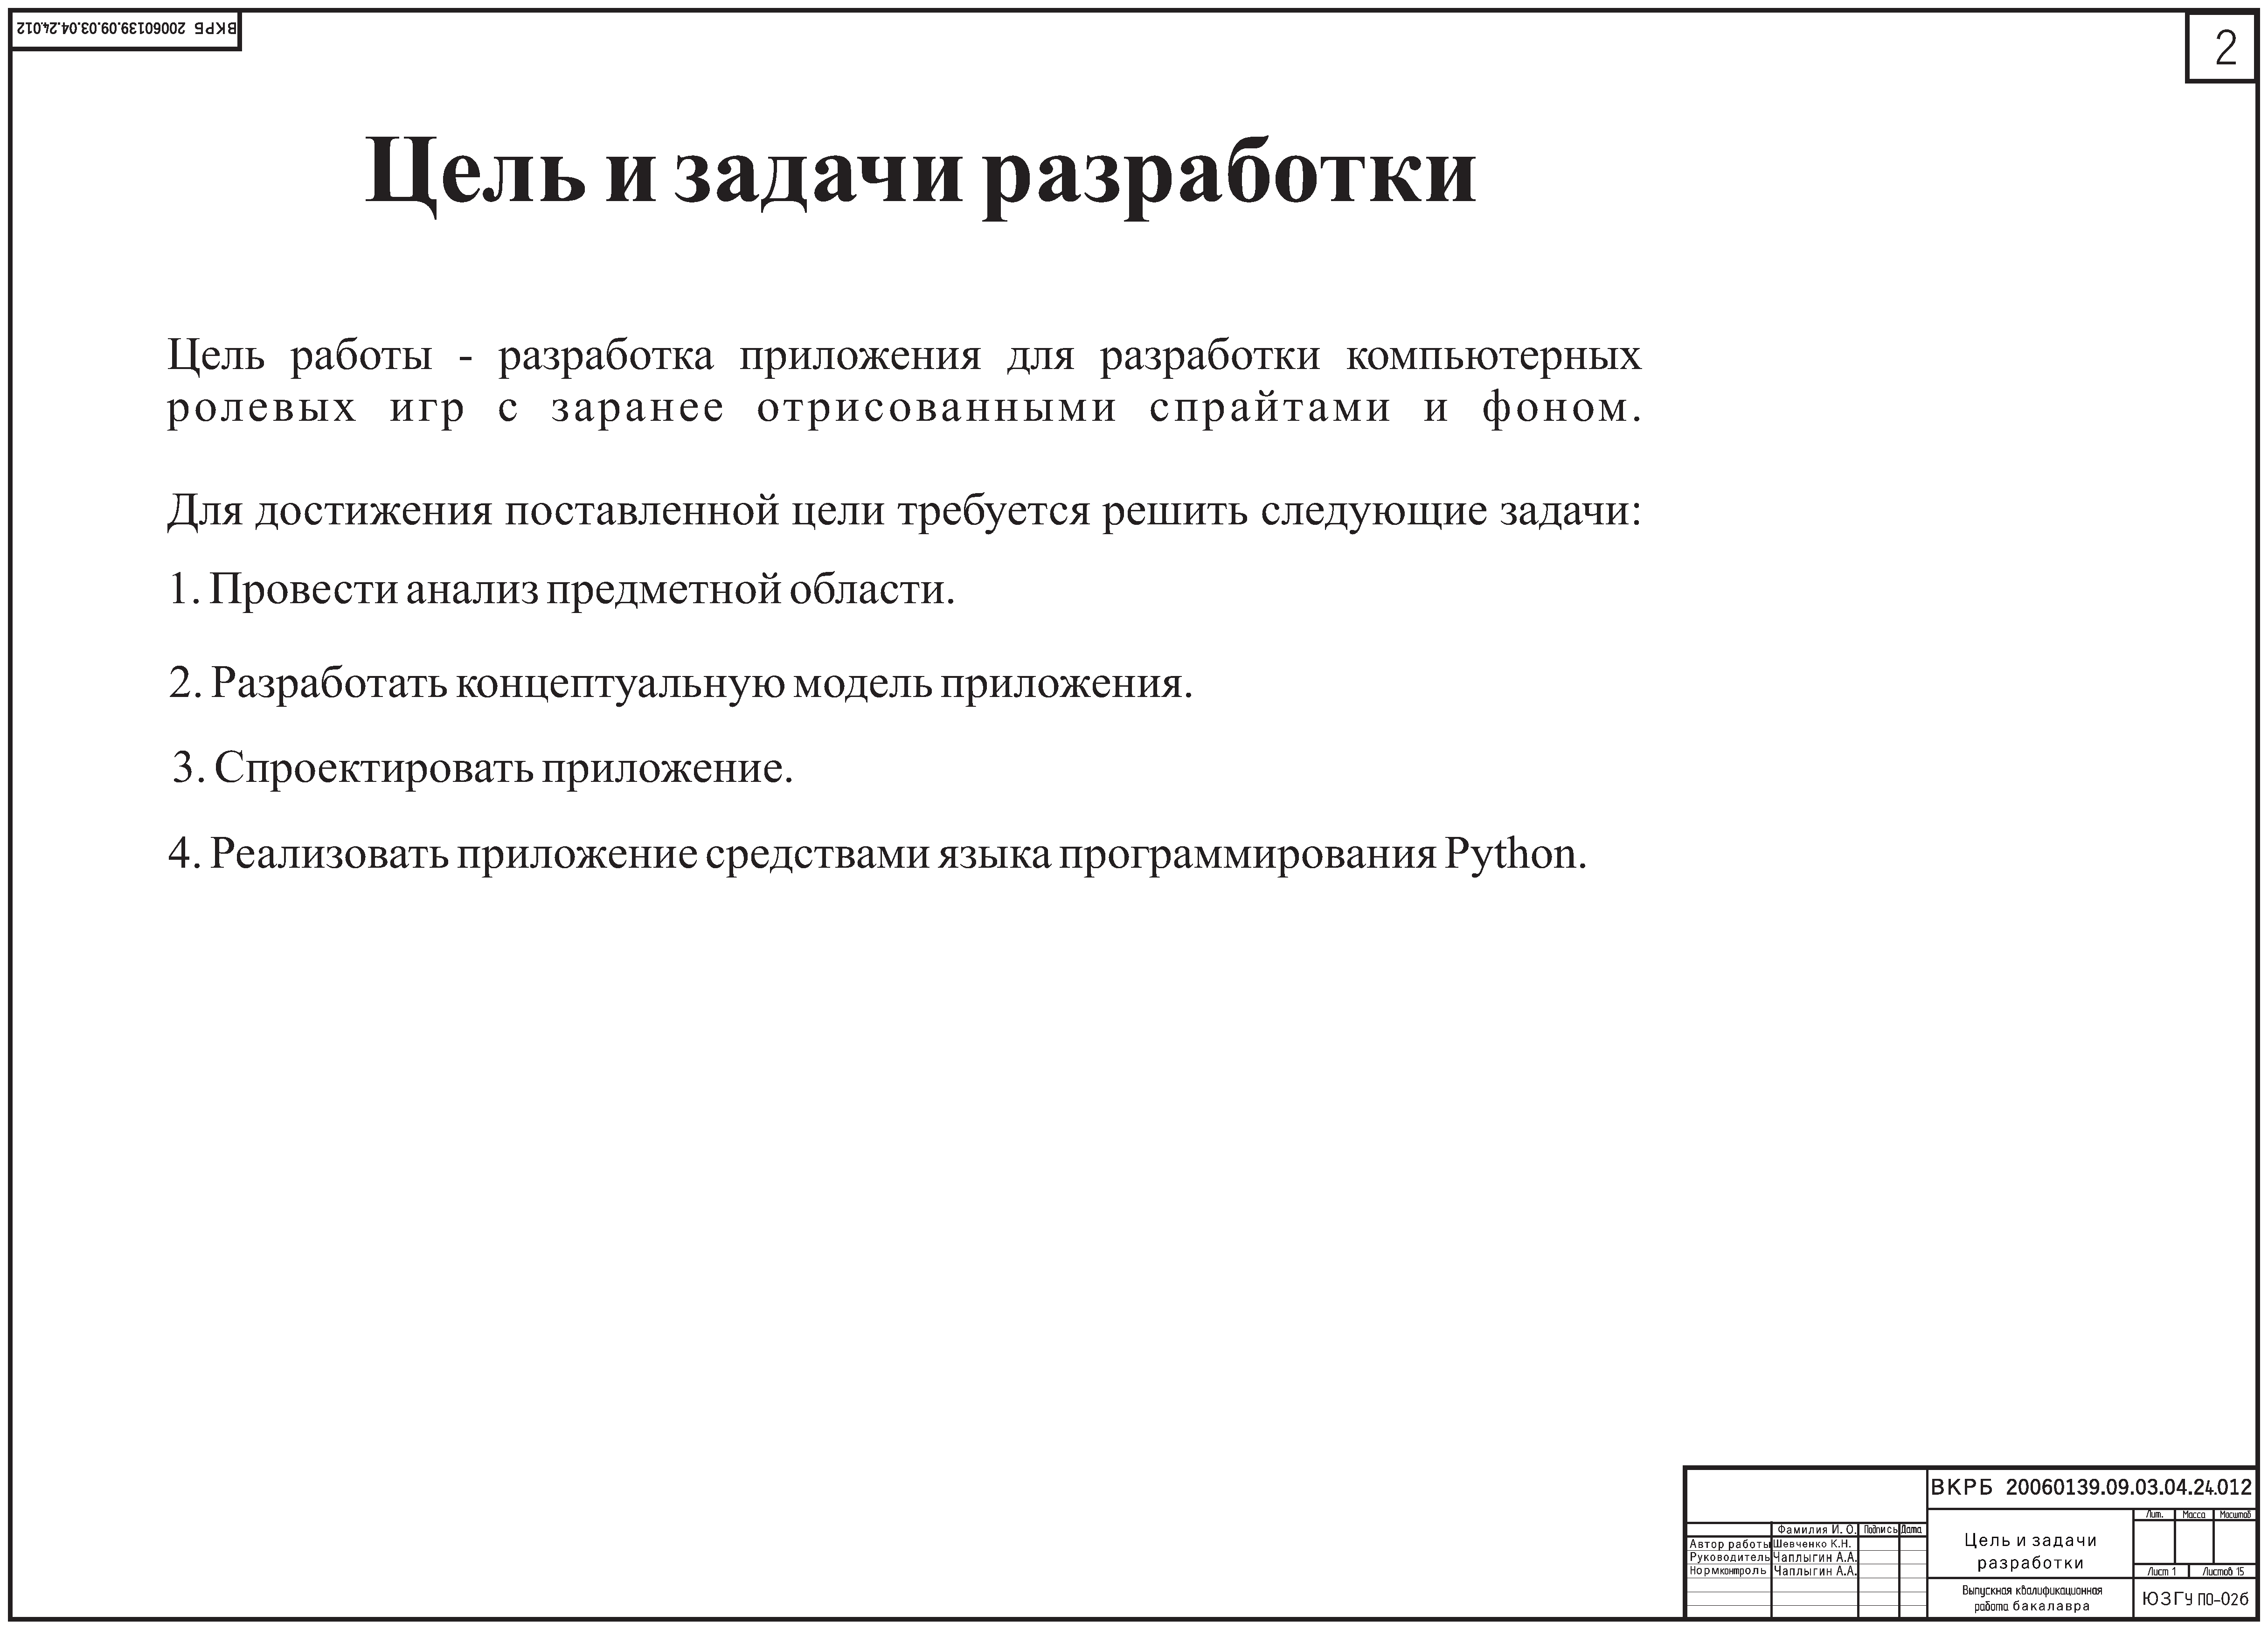
\includegraphics[width=0.82\linewidth]{плакат_2.esp}
    \заголовок{Цель и задачи разработки}
    \label{плакат_2.esp:image}      
\end{плакат}

\begin{плакат}
    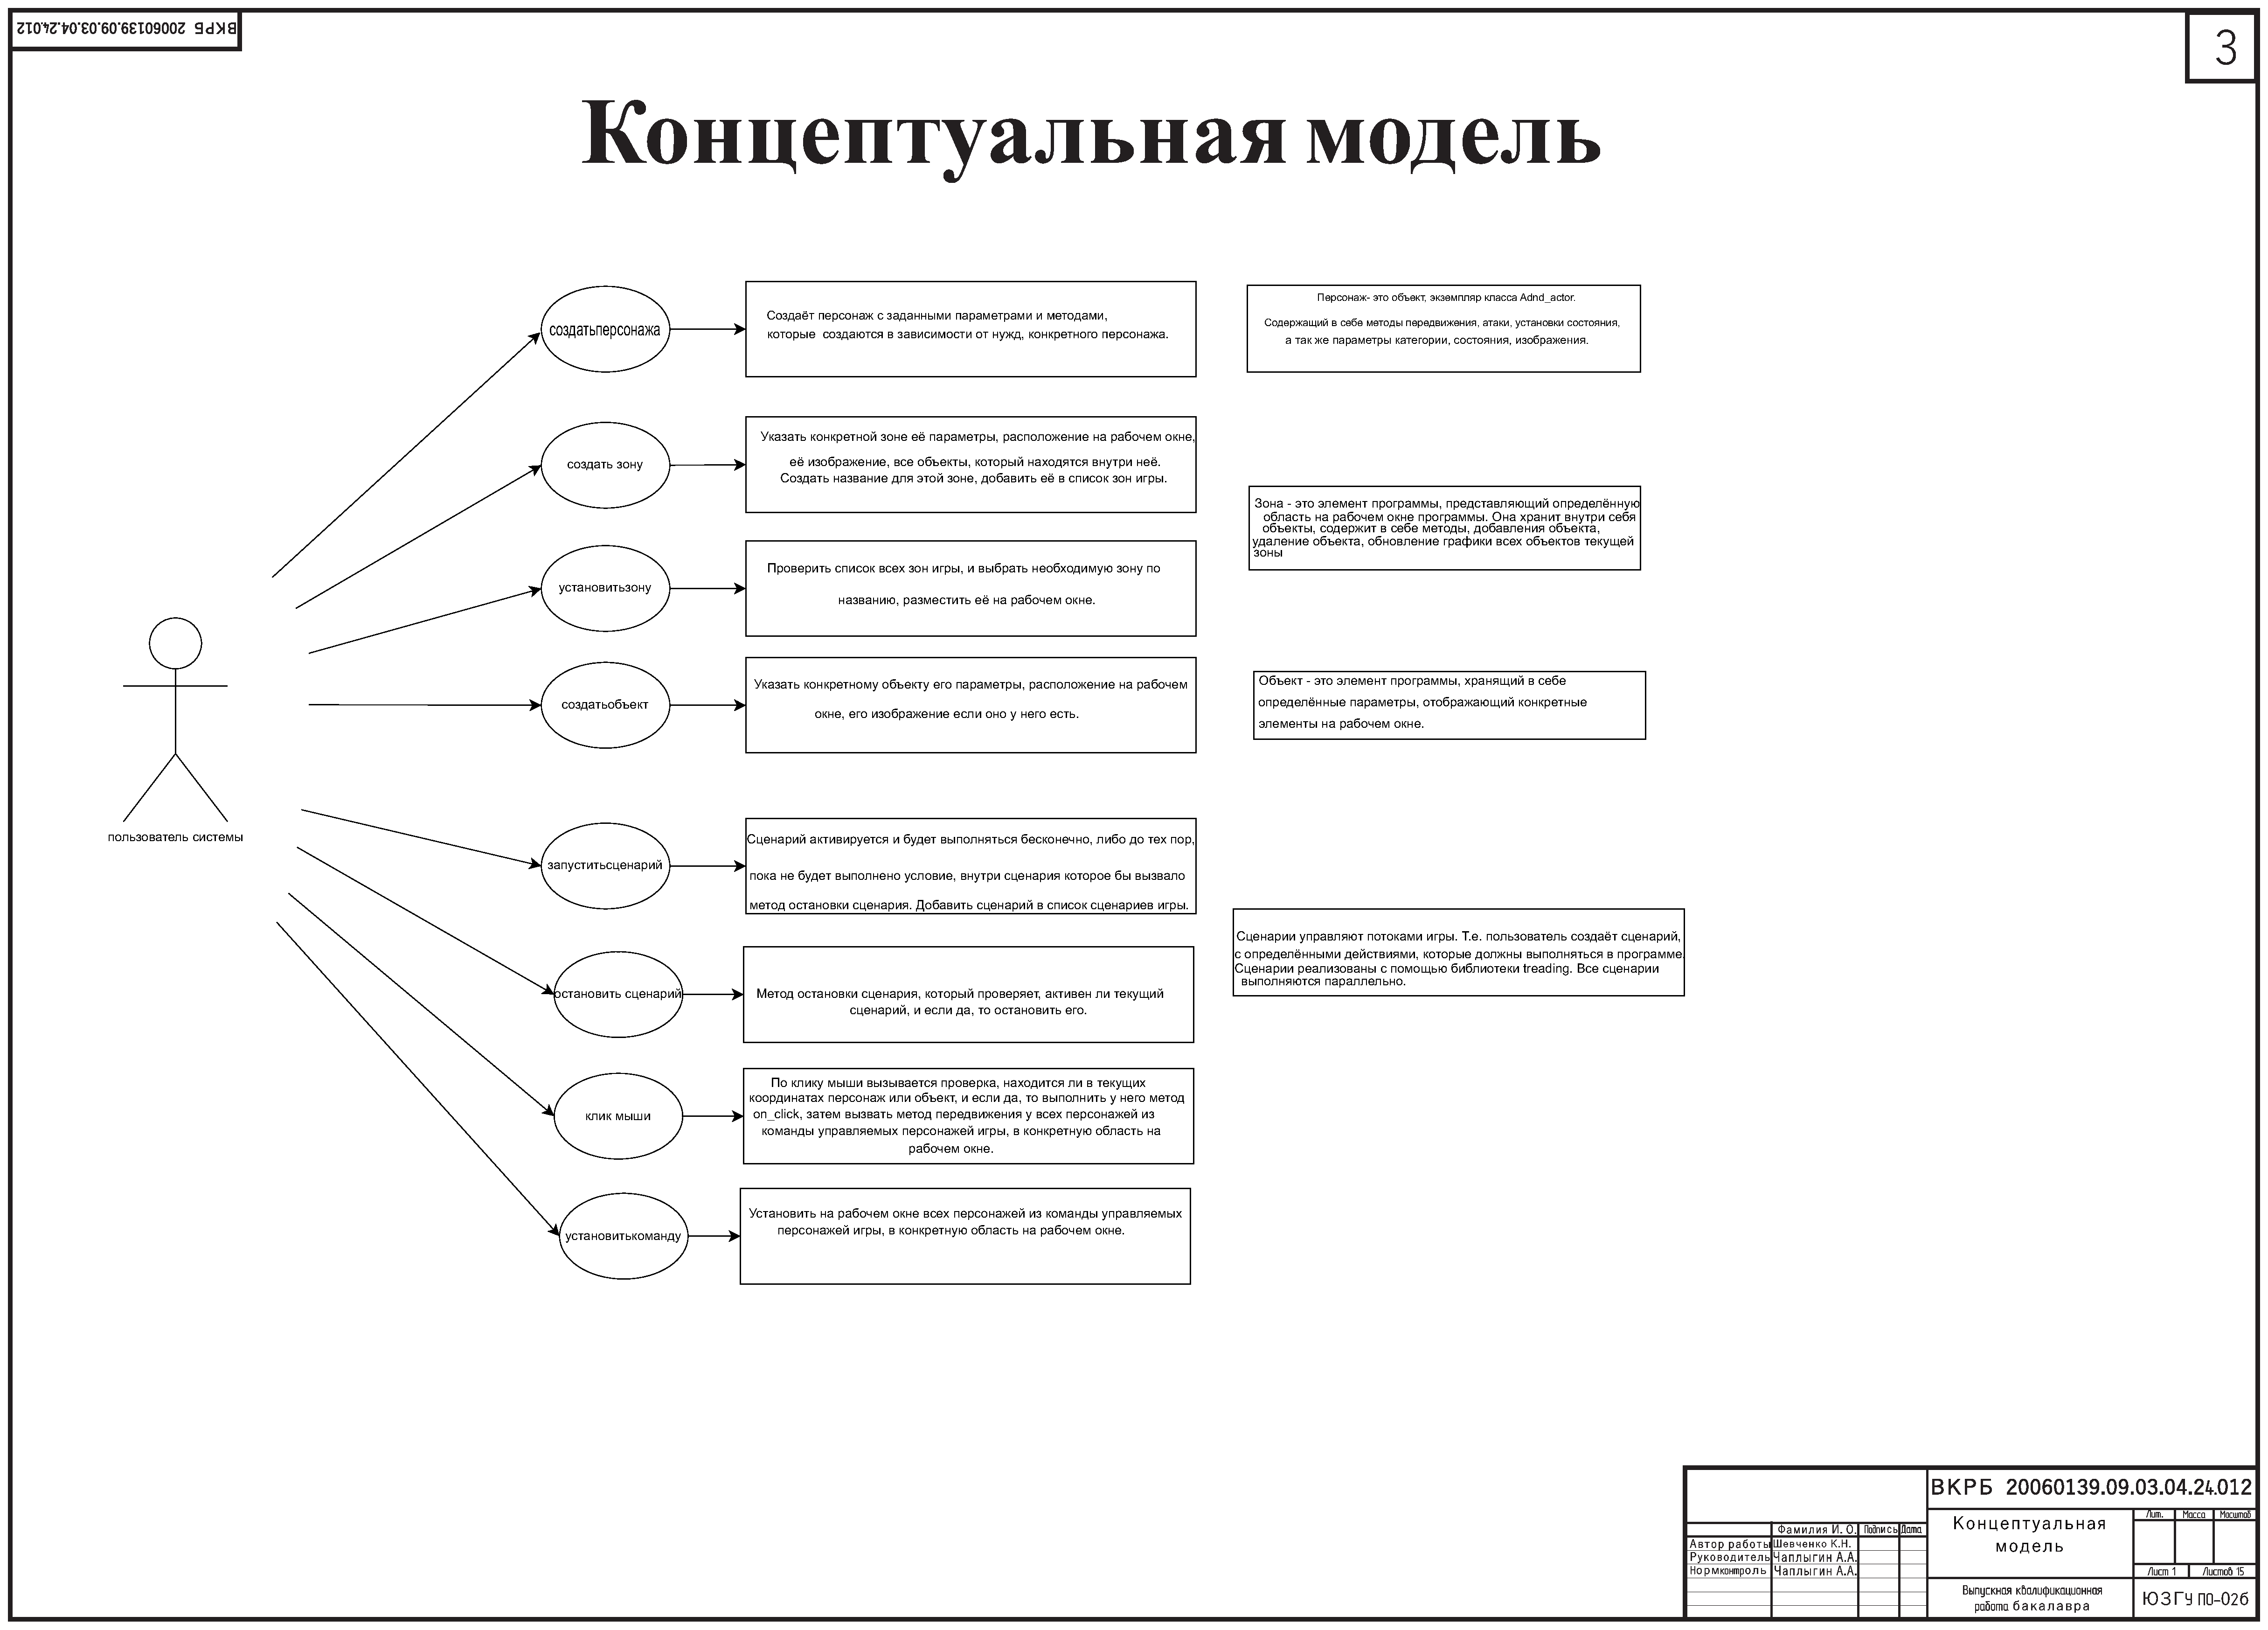
\includegraphics[width=0.82\linewidth]{плакат_3.esp}
    \заголовок{Концептуальная модель приложения}
    \label{плакат_3.esp:image}      
\end{плакат}

\begin{плакат}
	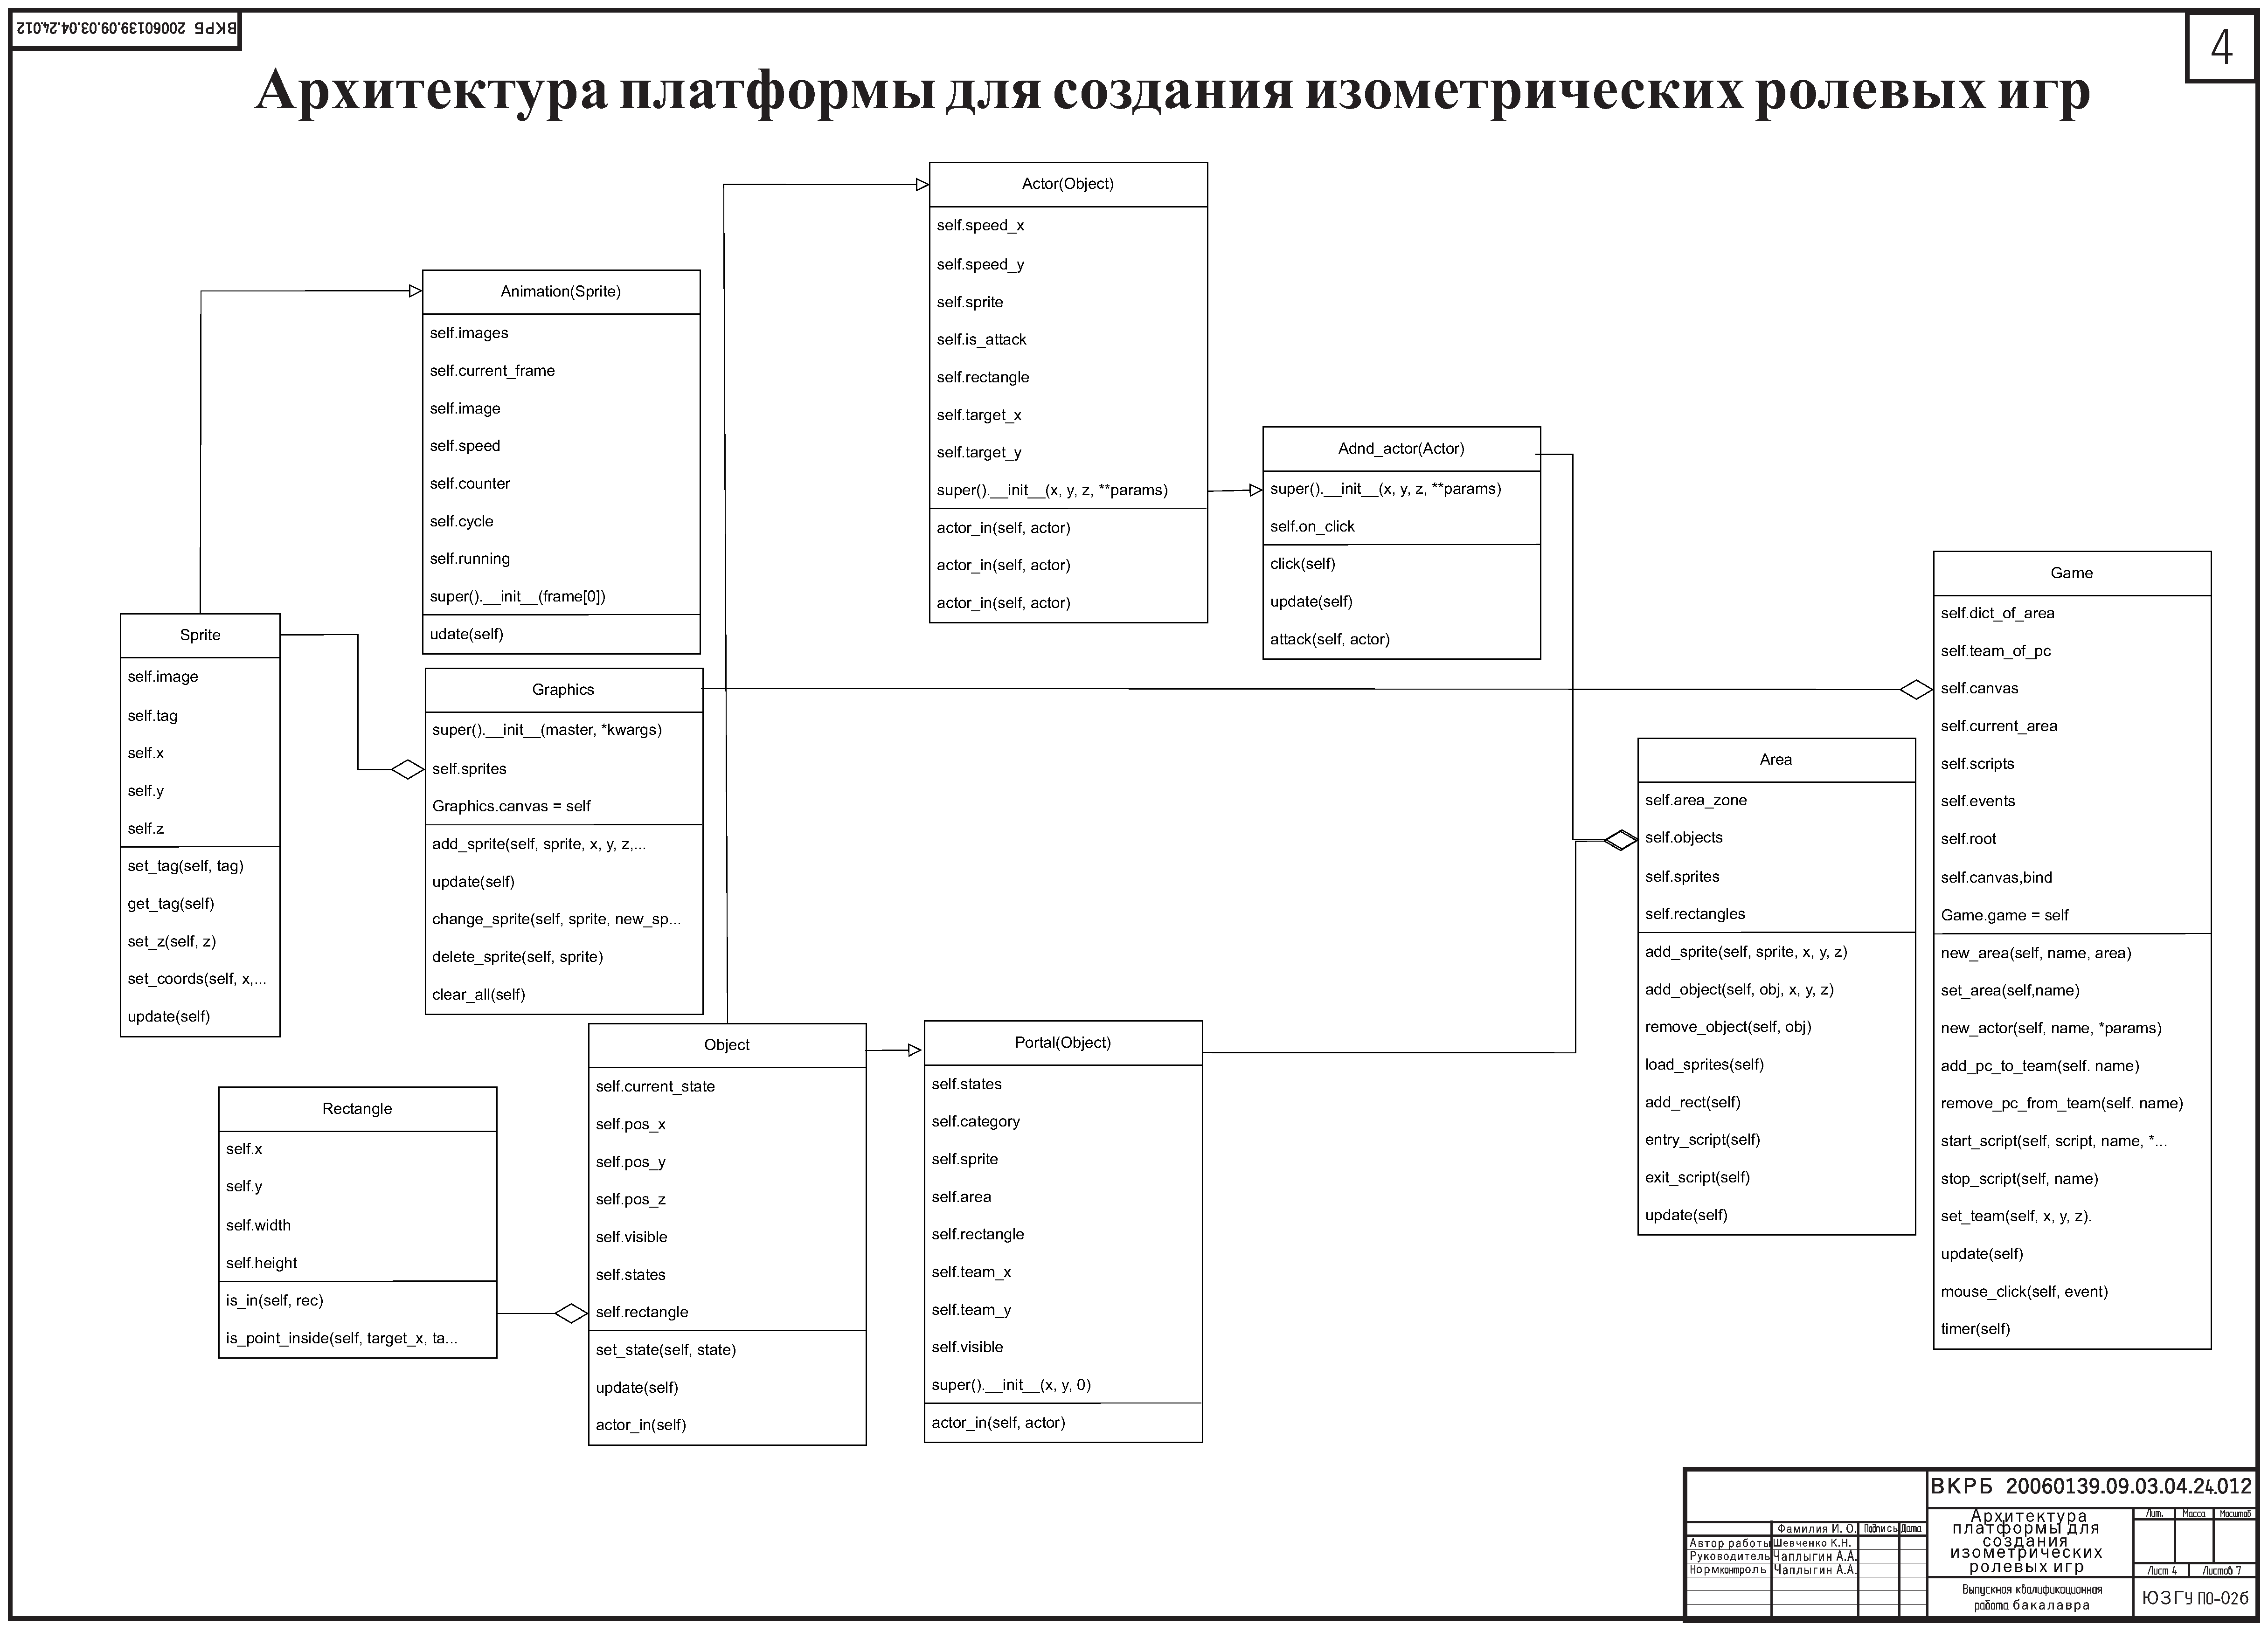
\includegraphics[width=0.82\linewidth]{плакат_4.esp}
	\заголовок{Диаграмма классов}
	\label{плакат_4.esp:image}      
\end{плакат}

\begin{плакат}
	
\includegraphics[width=0.82\linewidth]{плакат_5.esp}
	\заголовок{Модель работы сценариев}
	\label{плакат_5.esp:image}      
\end{плакат}

\begin{плакат}
	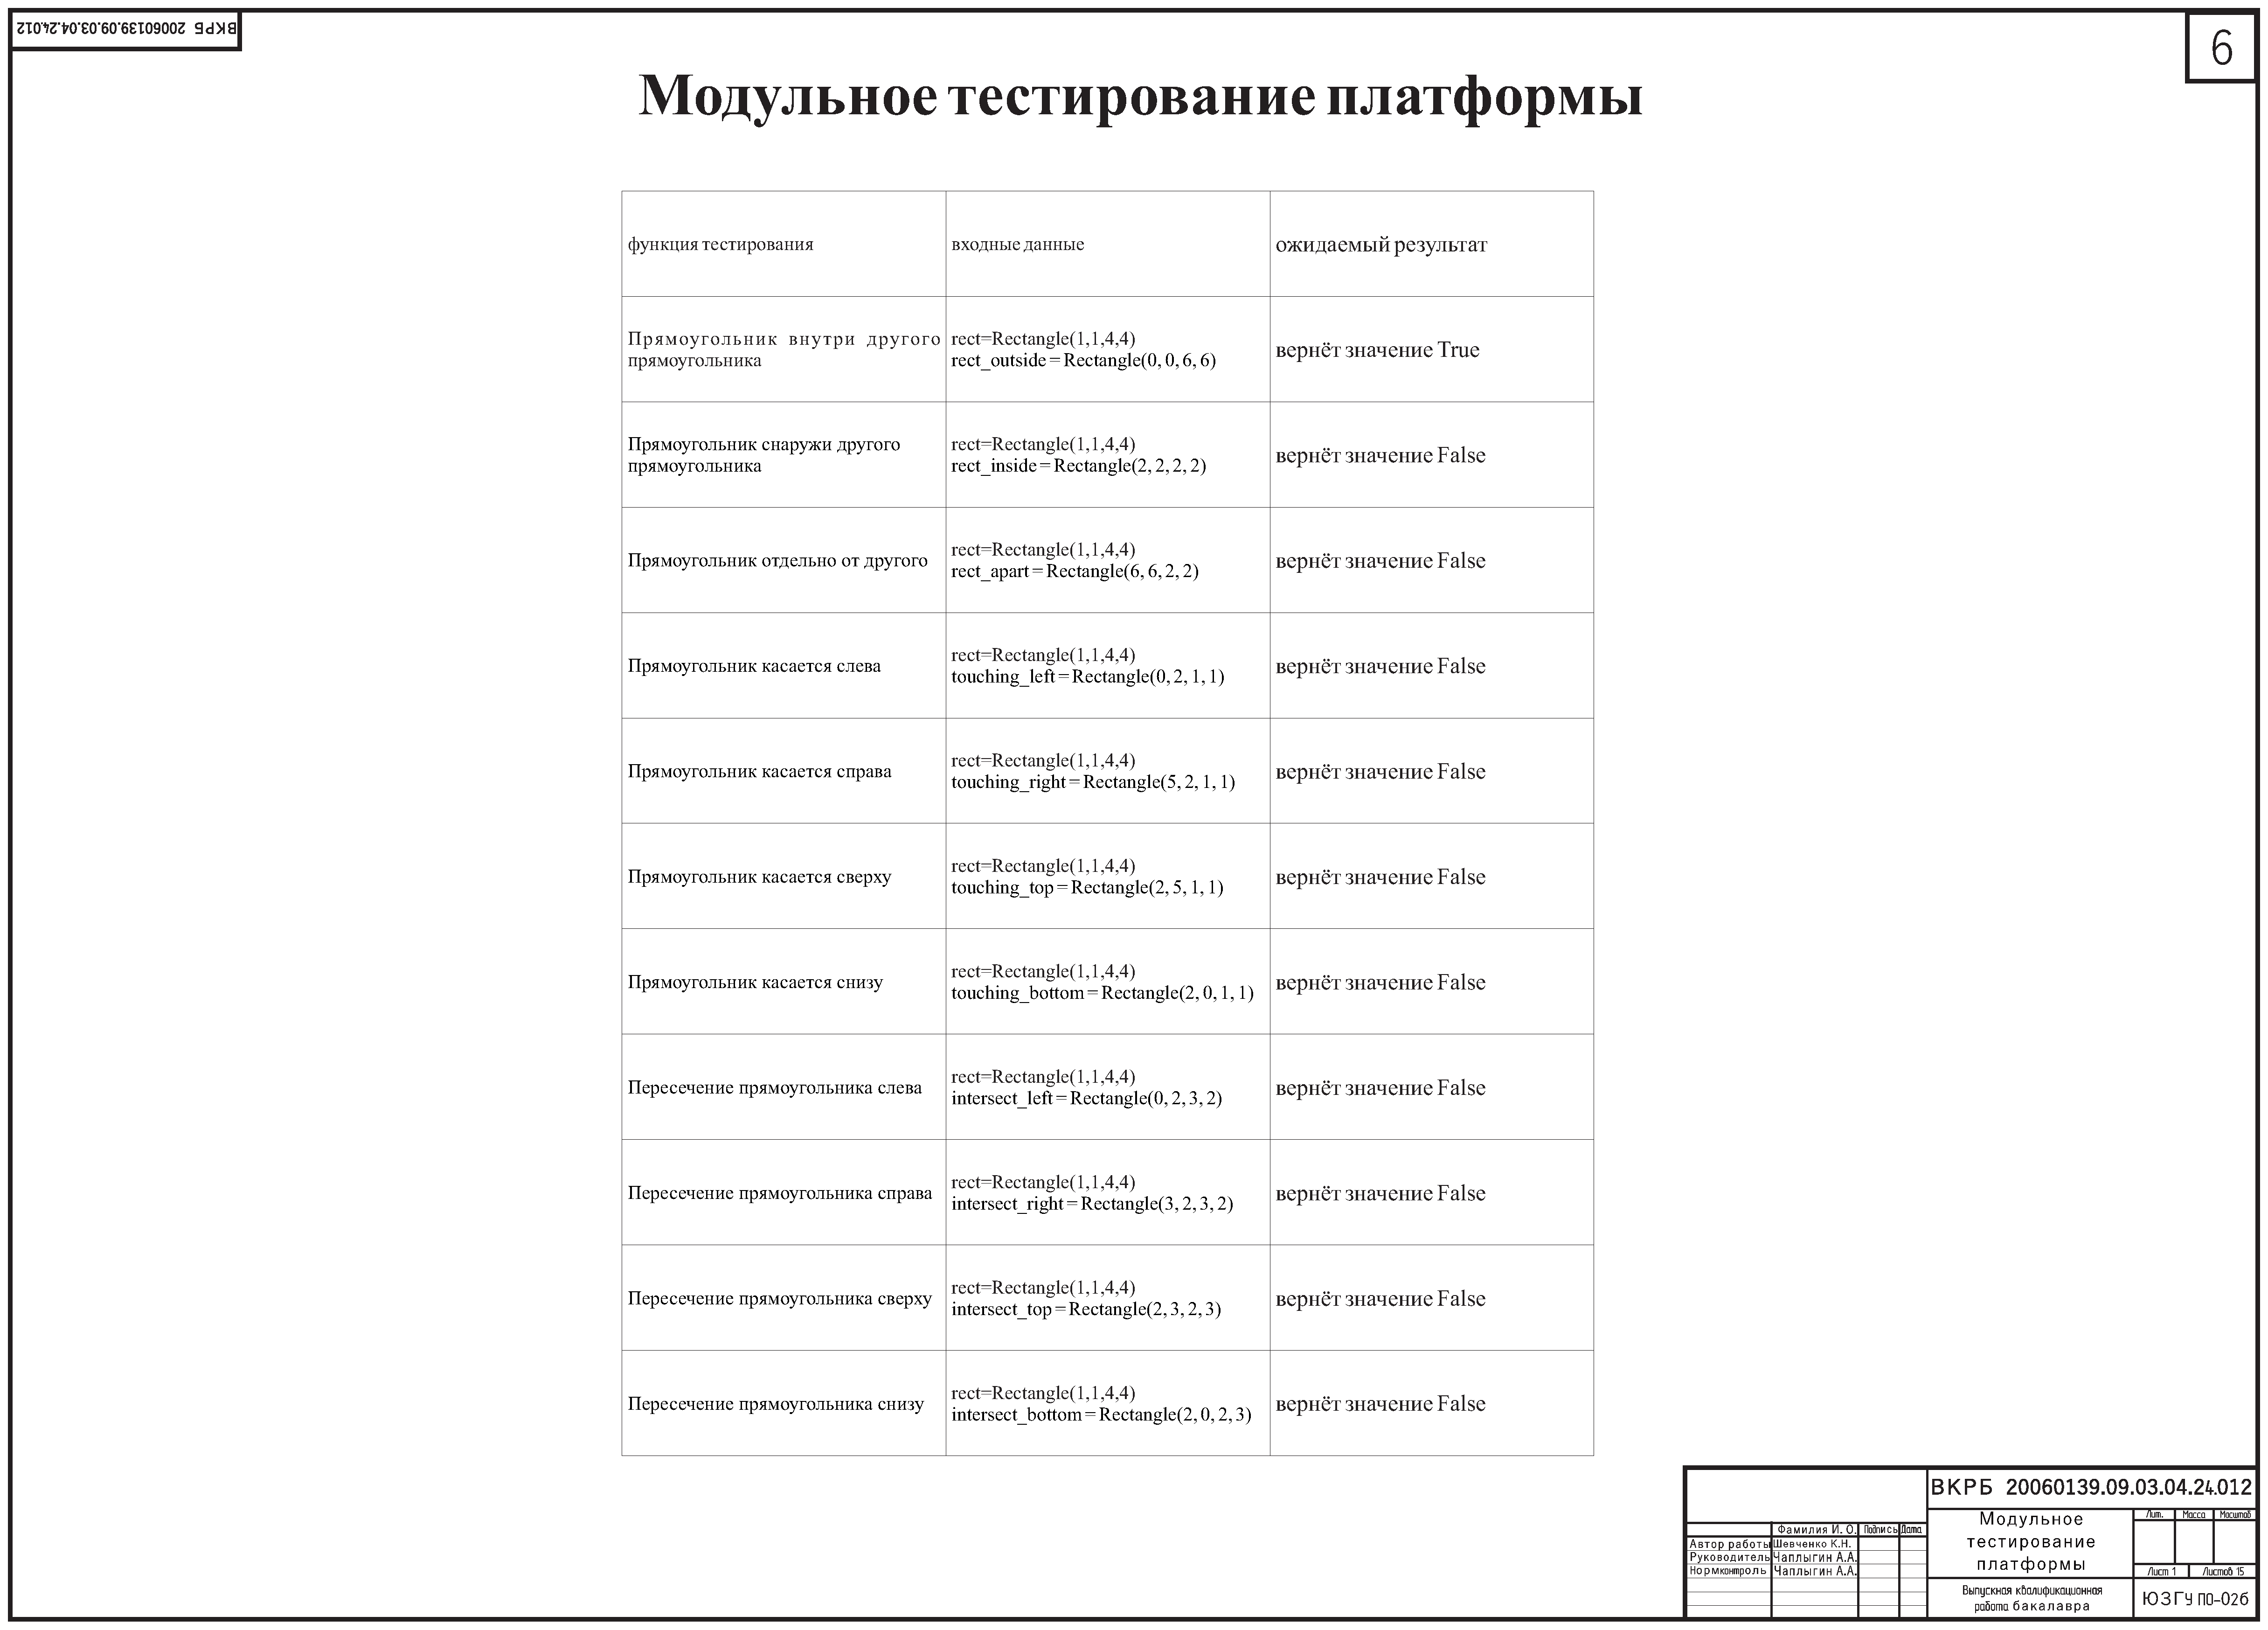
\includegraphics[width=0.82\linewidth]{плакат_6.esp}
	\заголовок{Модульное тестирование платформы}
	\label{плакат_6.esp:image}      
\end{плакат}

\begin{плакат}
	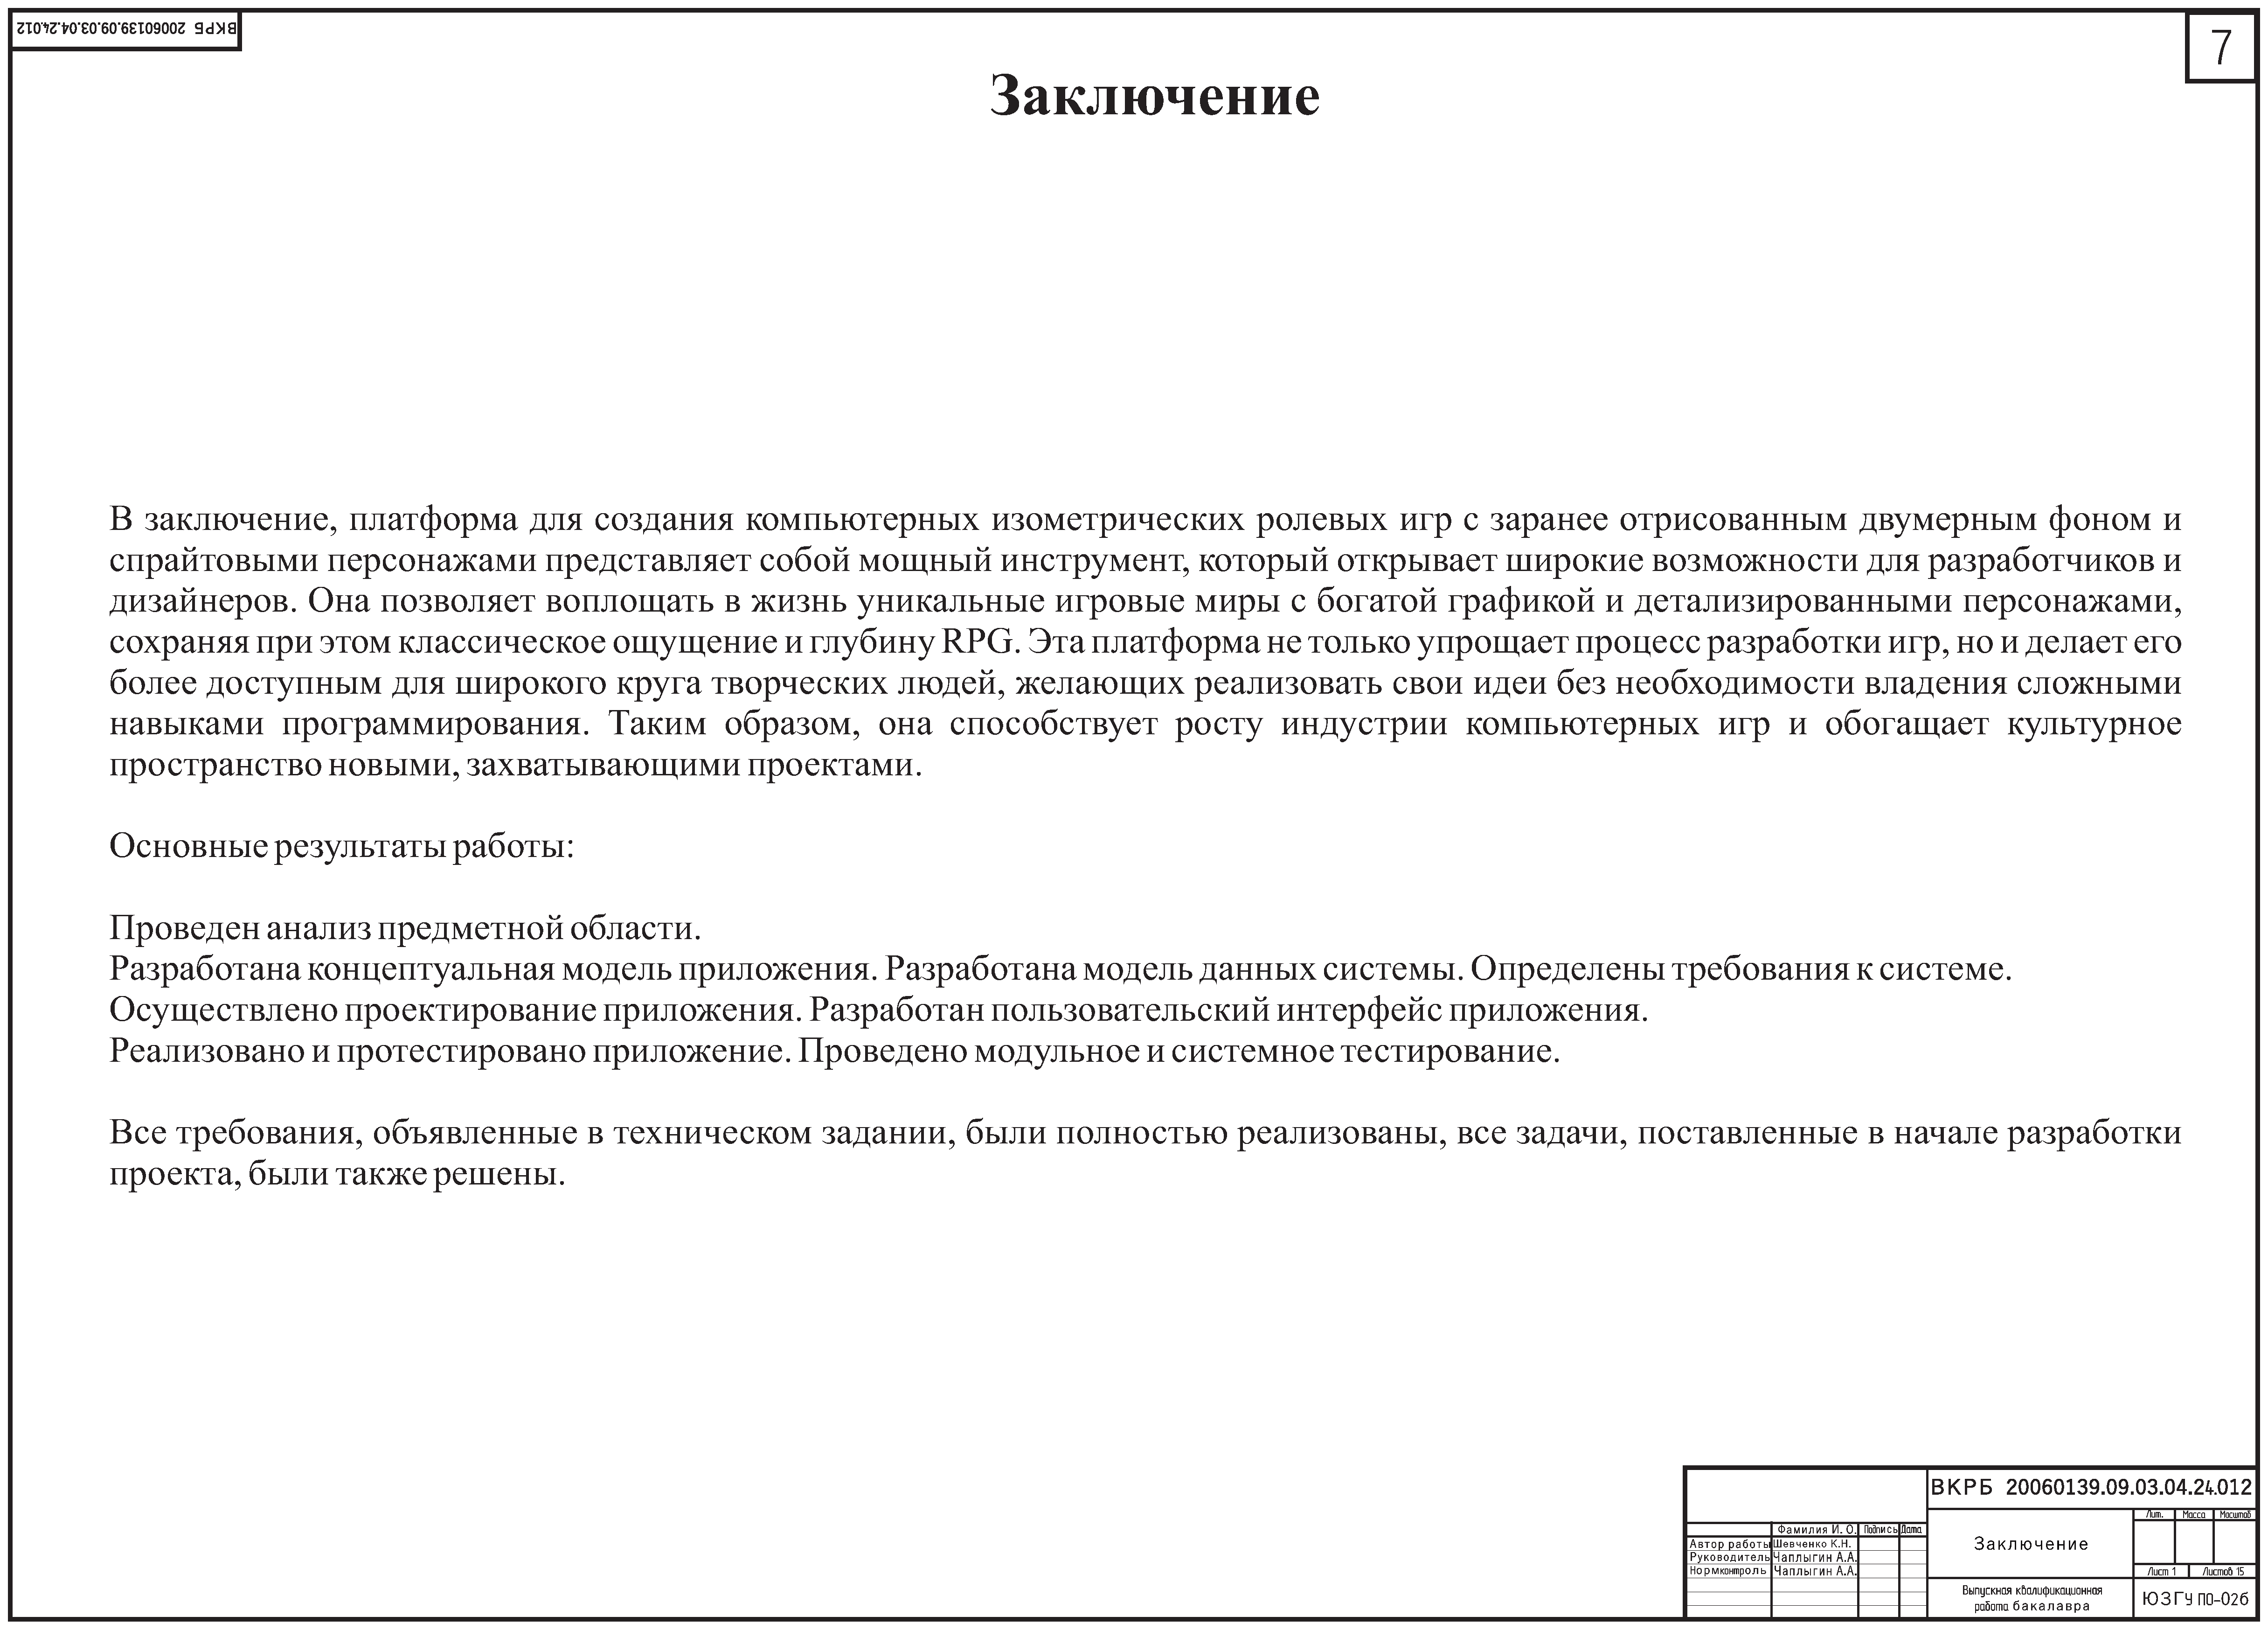
\includegraphics[width=0.82\linewidth]{плакат_7.esp}
	\заголовок{Заключение}
	\label{плакат_7.esp:image}      
\end{плакат}

\end{landscape}
